\documentclass{article}

\usepackage{polski}
\usepackage{titlesec}
\usepackage[english, polish]{babel}
\usepackage[utf8]{inputenc}
\usepackage{indentfirst}
\usepackage{listings}
\usepackage{graphicx}
\usepackage{float}

\graphicspath{ {./img/} }

\setcounter{secnumdepth}{4}
\setcounter{tocdepth}{4}

\title{Kryptografia - aplikacja Bob}
\date{\today}
\author{Marcin Szachun}

\begin{document}
\pagenumbering{gobble}
\maketitle
\newpage
\pagenumbering{arabic}

\tableofcontents
\newpage

\section{O aplikacji}
  Aplikacja ,,Bob'' jest konsolową aplikacją służcą do bezpośredniej i~natychmiastowej wymiany wiadomości pomiędzy 
  dwoma użytkownikami (zwanymi dalej ,,klient'' oraz ,,serwer'')
  Program został stworzony w języku programowania \emph{Python2}. Do stworzenia konsolowego interfejsu użytkownika
  została wykorzystana biblioteka \emph{ncurses} wraz z~biblioteką widgetów \emph{npyscreen}.
  Aplikacja pozwala na wymianę zarówno wiadomości tekstowych jak i~transmisję plików. Wykorzystywane aktualnie
  szyfrowanie (lub jego brak) może zostać w dowolnej chwili zmienione przez użytkownika. 

\section{Instrukcja obsługi aplikacji}
  \subsection{Uruchamianie aplikacji}
    Jak zostało wcześniej powiedziane aplikacja ,,Bob'' wykonana jest w~architekturze klient-serwer. W~związku 
    z~tym niezbędne jest uruchomienie dwóch instancji aplikacji: jednego serwera oraz klienta. Program należy 
    uruchomić z~konsoli, w~tym celu należy przejść do katalogu z aplikacją. Serwer uruchaminy jest przy pomocy 
    komendy:
      \lstset{language=sh,literate={--}{{-\,-}}1}
      \begin{lstlisting}
        ./bob.py --listen
      \end{lstlisting}
    Polecenie to uruchamia serwer, który oczekuje na połączenie pochodzące od klienta. Domyślnym portem na którym
    działa aplikacja oraz nasłuchuje serwer jest port \emph{1306}. Port ten można zmienić przy pomocy opcji 
    -{}-port:
      \lstset{language=sh,literate={--}{{-\,-}}1}
      \begin{lstlisting}
        ./bob.py --listen --port 8000
      \end{lstlisting}
    Po przygotowaniu serwera możliwe jest uruchomienie klienta. W tym celu należy przygotować nową konsolę oraz
    przejść do katalogu z aplikacją. Klient uruchamiany jest przy pomocy następującej komendy:
      \lstset{language=sh,literate={--}{{-\,-}}1}
      \begin{lstlisting}
        ./bob.py
      \end{lstlisting}
    Polecenie to powoduje próbę połączenia klienta z serwerem. Podobnie jak w~przypadku serwera domyślnie 
    wykorzystywanym portem jest \emph{1306}. Domyślnym hostem, z którym próbuje połączyć się klient jest
    \emph{localhost}. Zarówno domyślny port oraz host może zostać zmieniony przez użytkownika:
      \lstset{language=sh,literate={--}{{-\,-}}1}
      \begin{lstlisting}
        ./bob.py --port 8000 192.168.1.100
      \end{lstlisting}

  \subsection{Interfejs aplikacji}
    Na zrzutach ekranowych (rys. \ref{SERVER_INTERFACE} oraz rys. \ref{CLIENT_INTERFACE}) przedstawiono interfejs
    aplikacji  zaraz po uruchomieniu oraz w trakcie działania.  Wyróżnione elementy zostały opisane poniżej.
    \begin{figure}[tp]
        \centering
        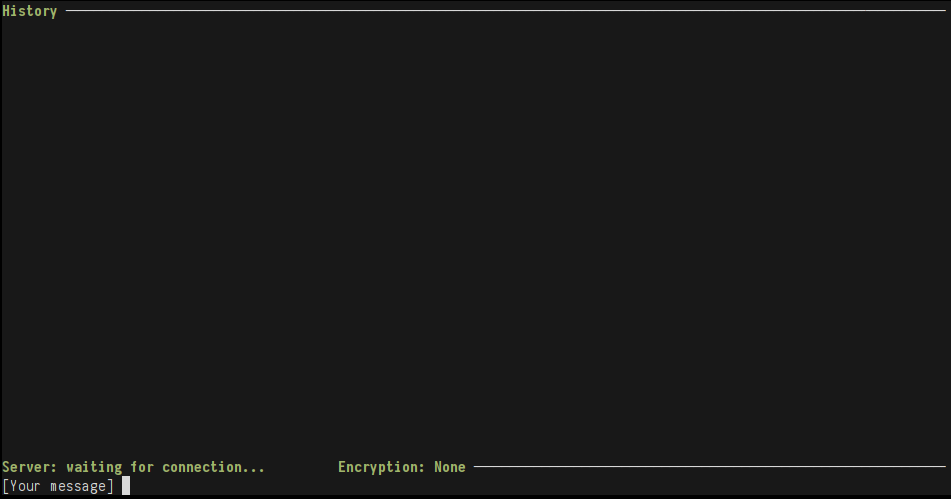
\includegraphics[scale=0.4]{podstawowy_interfejs_po_uruchomieniu_serwer}
        \caption{Interfejs aplikacji ,,Bob'' uruchomionej jako serwer}
        \label{SERVER_INTERFACE}
    \end{figure}
    \begin{figure}[tp]
        \centering
        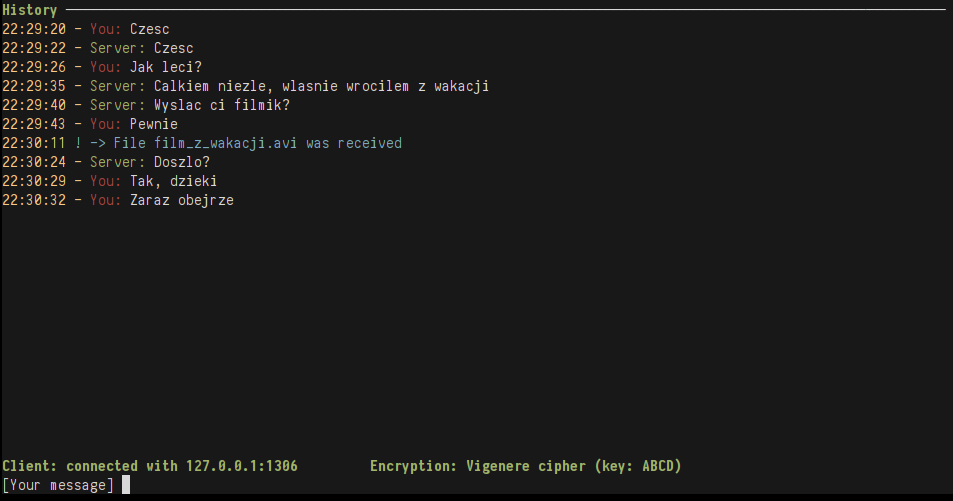
\includegraphics[scale=0.4]{interfejs_podczas_dzialania_klient}
        \caption{Interfejs aplikacji ,,Bob'' w trakcie działania jako klient}
        \label{CLIENT_INTERFACE}
    \end{figure}
    \subsubsection{Pasek stanu}
      Pasek stanu zawiera informacje na temat aktualnego statusu aplikacji. Znajdują się tutaj informacje na temat
      połączenia oraz aktualnie wykorzystywanego szyfrowania
    \subsubsection{Okienko do wpisywania wiadomości}
      Domyślnie aktywne po uruchomieniu aplikacji. Możliwe jest tutaj wpisanie treści wiadomości do przekazania
      rozmówcy. Po wpisaniu wiadomości jej wysłanie odbywa się po wciśnięciu klawisza \emph{Enter}
    \subsubsection{Historia rozmowy}
      W oknie tym wyświetlone są wszystkie wiadomości odebrane oraz wysłane. Każda wiadomość opisana jest godziną
      wysłania (odebrania) oraz nadawcą. Możliwe jest aktywowanie okna historii poprzez naciśnięcie klawisza
      \emph{Tab}. Po aktywowaniu, możliwe jest wybieranie wiadomości. Po naciśnięciu klawisza \emph{Enter} na 
      wybranej wiadomości wyświetlone zostanie okienko ze szczegółami wiadomości. Możliwe jest tutaj sprawdzenie
      szyfrowania, które zostało użyte do wysłania wiadomości oraz podejrzenie powstałego szyfrogramu oraz tekstu
      jawnego.

      Oprócz wysłanych oraz odebranych wiadomości w oknie historii rozmowy wyświetlane są również informacje na 
      temat odebranych oraz wysłanych plików. Podobnie jak w przypadku wiadomości możliwe jest wybranie dowolnego
      z tych wpisów oraz po naciśnięciu klawisza \emph{Enter} podejrzenie szczegółów transmisji plików.

    \begin{figure}[H]
        \centering
        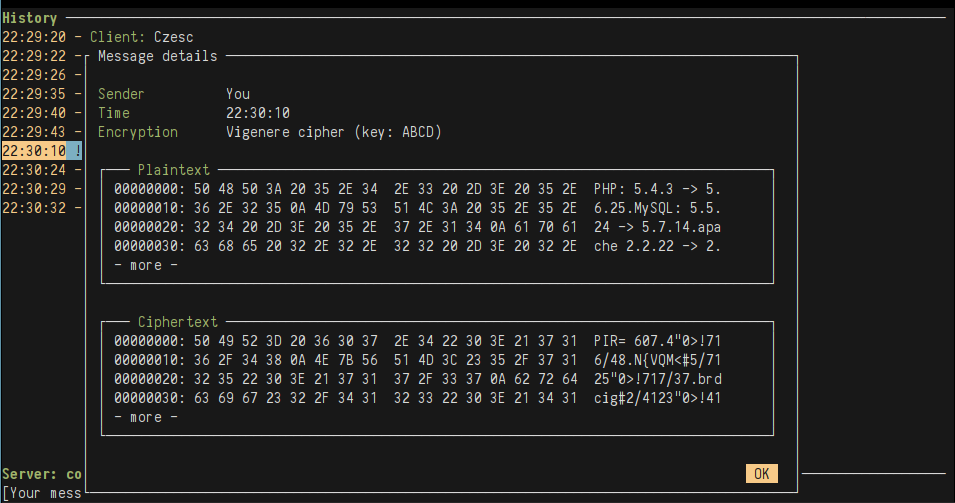
\includegraphics[scale=0.4]{szczegoly_transferu_pliku}
        \caption{Okienko przedstawiające szczegóły transferu pliku}
        \label{FILE_TRANSFER_DETAILS}
    \end{figure}

      W zależności od wykorzystywanego szyfrowania oraz od tego czy wybrana została wiadomość czy transfer pliku,
      szyfrogram oraz tekst jawny mogą zostać przedstawione w postaci zwykłego tekstu lub w postaci szesnastkowej.

    \subsubsection{Menu aplikacji}
      Menu aplikacji otwierane jest po naciśnięciu klawiszy \emph{CTRL + X}

    \begin{figure}[H]
        \centering
        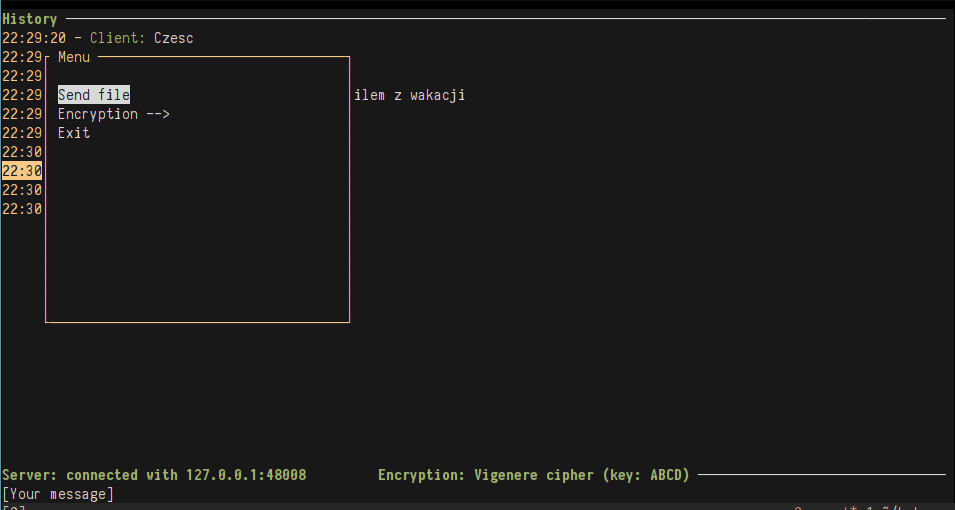
\includegraphics[scale=0.4]{menu_aplikacji}
        \caption{Menu aplikacji}
        \label{APPLICATION_MENU}
    \end{figure}

    \paragraph{Wysyłanie pliku}
      Po wybraniu opcji \emph{Send file} możliwe jest wysłanie pliku do rozmówcy. W wyświetlonym oknie należy za
      pomocą strzałek wybrać odpowiedni plik, po czym zatwierdzić wybór klawiszem \emph{Enter}. W tym momencie
      rozmówca zostaje poproszony o akceptację transferu pliku, oraz wskazanie lokalizacji zapisu pliku, przy 
      pomocy analogicznego okna dialogowego. Po akceptacji rozpoczna się transmisja pliku, której postęp
      przedstawiony jest w~wyświetlonym okienku.

    \begin{figure}[h]
        \centering
        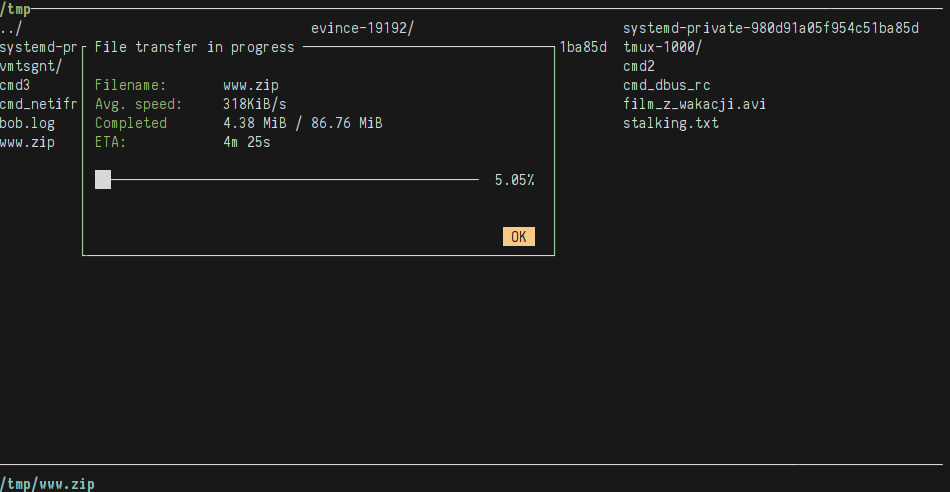
\includegraphics[scale=0.4]{transfer_pliku}
        \caption{Okieno pokazujące postęp transmisji pliku}
        \label{FILE_TRANSFER_PROGRESS}
    \end{figure}

    \paragraph{Zmiana sposobu szyfrowania}
      Przy pomocy opcji \emph{Encryption} możemy wybrać sposób szyfrowania przesyłanych wiadomości oraz plików.
      Po wybraniu tej opcji w kolejnym menu zaprezentowane są dostępne sposoby szyfrowania. Po wybraniu dowolnego z
      nich wyświetlone zostaje okienko konfiguracji szyfrowania. W zależności od wybranego algorytmu należy podać
      odpowiedni klucz. Po zatwierdzeniu przyciskiem \emph{OK} szyfrowanie będzie aplikowane do wysłanych oraz
      odebranych wiadmości. Informacja o wykorzystywaniu szyfrowania zostaje wysłana do rozmówcy, dzięki czemu nie
      jest konieczne ponowne konfigurowanie algorytmu, zostaje on ustawiony automatycznie

    \begin{figure}[H]
        \centering
        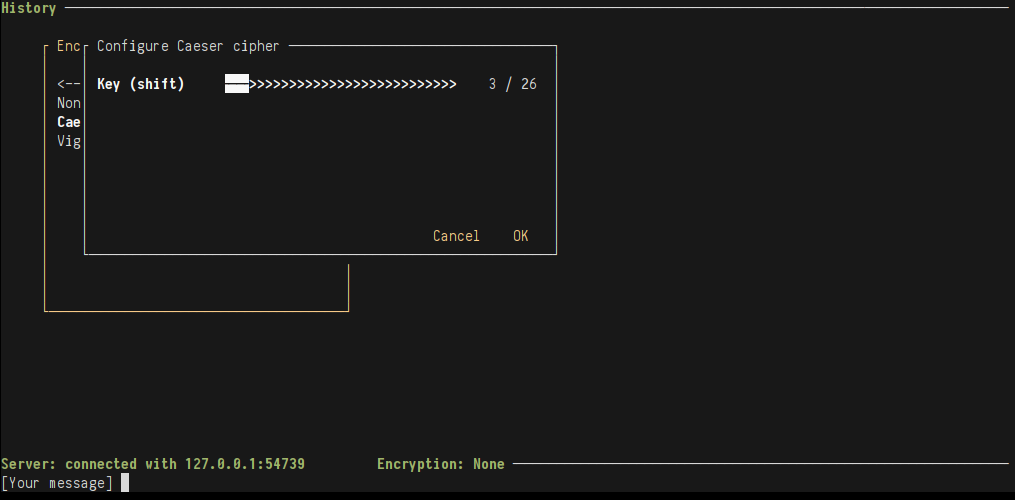
\includegraphics[scale=0.4]{caesar_cipher_configuration}
        \caption{Okienko konfiguracji szyfru Cezara}
        \label{CIPHER_CONFIGURATION}
    \end{figure}

    \paragraph{Wyjście z aplikacji}
      Po wybraniu opcji \emph{Exit} aplikacja zostaje zamknięta. Do rozmówcy zostaje wysłana informacja o 
      zerwaniu połączenia, w~związku z czym jego aplikacja również zostaje zamknięta

  \section{Szczegóły implementacji algorytmów szyfrowania}
      

\end{document}
